\section{Spannungsausbreitung\label{spannung:section:Oedometer - Versuch}}
\rhead{Oedometer - Versuch}
Beim Oedometer - Versucht hat man einen Stahlring mit einer Filterplatte am Boden.
In diesen Stahlring wird eine Bodenprobe eingefüllt.
Anschliessend wir mit einer Platte das Bodenmaterial mit einer ansteigenden Kraft belastet.

Die Probe wird sich so verdichten. Das Volumen nimmt ab.
Der Stahlring verhindert ein seitliches ausbrechen oder entweichen der Bodenprobe.
Die Dehnung auf der Seite beträgt somit 0.
Mit dem Wert der Kraft und der Fläche lässt sich die Spannung berechnen.
Anhand der Volumenabnahme errechnet man die Dehnung.
Aus diesen Werten lässt sich wiederum das E-Modul bestimmen.
Beim Oedometer Versuch ist das E-Modul als $E_{OED}$ bezeichnet.

Das $E_{OED}$ hat man speziell in der Geotechnik.
Dies aufgrund der speziellen Situation wo man sich mit dem infinitesimalen Würfel befindet.
Mit dem Stahlring, der verhindert das Material seitlich entweichen kann hat man ganz ähnliche Verhältnisse wie tief im Untergrund.
Auch dort kann das Material bei einer Belastung nicht seitlich entweichen.

Wichtig ist nochmals zu betonen, dass alle diese beschriebenen Berechnungen ausschliesslich im linear-elastischen Materialverhalten funktionieren.
So ist es auch beim Oedometer - Versuch.
Den Versuch kann man auf einem $\sigma$ und $\varepsilon$ Diagramm abtragen.

\begin{figure}
	\centering
	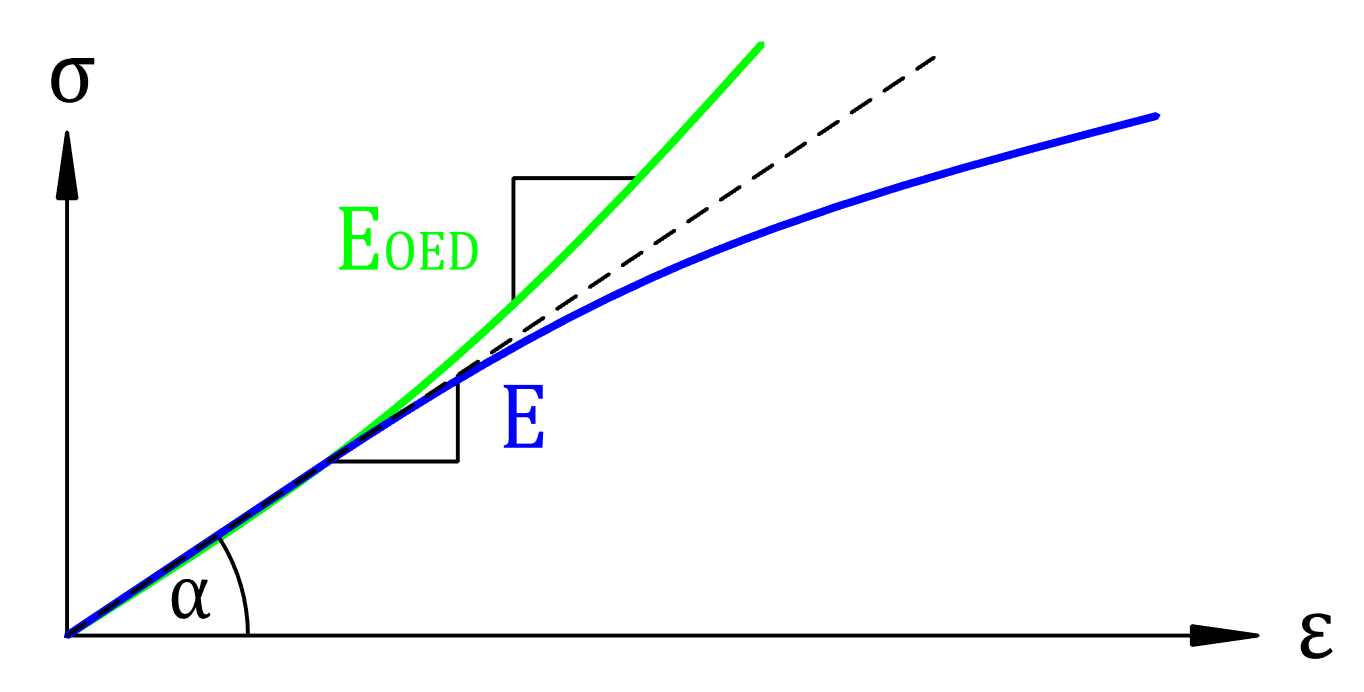
\includegraphics[width=0.5\linewidth,keepaspectratio]{papers/spannung/Grafiken/DiagrammOedometer-Versuch.png}
	\caption{Diagramm Oedometer - Versuch}
	\label{fig:Diagramm Oedometer - Versuch}
\end{figure}

Bei einem Versuch mit anderem Baumaterial wie beispielsweise Holz nimmt die Dehnung im Laufe des Versuchs stärker zu, obwohl weniger Spannung abgetragen wird.
Bei den meisten Böden ist dies anders. Durch die Komprimierung nimmt der Boden mehr Spannung auf, und verformt sich zugleich weniger stark.

Man kann die Dehnung in unsere vereinfachte Matrix einsetzen. Das E-Modul ersetzt man mit dem $E_{OED}$.

\[
\overbrace{\sigma_{11}-\sigma_{33}}^{q}
=
\frac{3E}{2(1+\nu)} \overbrace{\frac{2}{3}(\varepsilon_{11} - 0)}^{\varepsilon_{\nu}}
\]

\[
\overbrace{\frac{\sigma_{11}+2\sigma_{33}}{3}}^{p}
=
\frac{E}{3(1-2\nu)} \overbrace{(\varepsilon_{11} - 2\cdot0)}^{\varepsilon_{s}}
\]

\[
\begin{pmatrix}
	\sigma_{11}-\sigma_{33} \\
	\sigma_{11}+2\sigma_{33}
\end{pmatrix}
=
\begin{bmatrix}
	\frac{E_{OED}}{(1+\nu)} &                        0 \\
	                      0 & \frac{E_{OED}}{(1-2\nu)}
\end{bmatrix}
\begin{pmatrix}
	\varepsilon_{11}\\
	\varepsilon_{11}
\end{pmatrix}
\]

An einem geeigneten Punkt, wo man noch im linear-elastischen Materialverhalten ist, kann man nun das $E_{OED}$ abtragen.
Es wird nur ein Delta betrachtet um $E_{OED}$ zu berechnen.
Man darf die Dehnung nicht über den gesamten Verlauf betrachten um $E_{OED}$ zu berechnen.

Mit diesem ermittelten E-Modul kann man nun weitere Berechnungen für die Geotechnik durchführen.
